\documentclass[11pt,a4paper]{article}

\usepackage{latexsym}
\usepackage[german]{babel}
\usepackage[utf8]{inputenc}
\usepackage{amsmath}
\usepackage{graphicx}
\usepackage[colorinlistoftodos]{todonotes}
\usepackage{natbib}
\usepackage{multirow}
\usepackage{url}
\usepackage{microtype}
\usepackage{paralist}
\usepackage{tabularx}
\usepackage{booktabs}
\usepackage{covington}
\usepackage{verbatim}
\usepackage{amsmath}
\usepackage{csquotes}
\usepackage{algorithm}
\usepackage{algorithmic}
\usepackage[skip=4pt]{caption}
\usepackage[hyperref]{acl2018}
\usepackage{rotating}
\usepackage{afterpage}
\usepackage{pdflscape}

\newcommand{\lang}[1]{\textit{#1}}
\newcommand{\action}[1]{\texttt{#1}}

%\aclfinalcopy

\title{Projekt Sprachtechnologie\\Projektbericht}

\author{Fynn Schröder\qquad (7003971)\\Marcel Kamlot\qquad Matr.Nr\\Gregor Billing\qquad(6808038)}

\date{20.09.2018}

\begin{document}
\maketitle

\begin{abstract}
Toller Kram\todo[inline]{todo}
\end{abstract}

\section{Einleitung und Aufgabenstellung}
\label{sec:introduction}
In diesem Projekt haben sich die Autoren mit Wortflexion, also der Wortbildung durch Anpassung an die grammatische Funktion innerhalb des Satzes befasst. Im Deutschen umfasst dies üblicherweise die Deklination von Substantiven und Adjektiven nach Kasus, Numerus und Genus sowie die Konjugation von Verben.
Andere Sprachen können jedoch anderen Flexionsparadigma unterliegen, und so wurde von Anfang an darauf geachtet, ein möglichst sprach-neutrales System zu entwerfen, das sich unabhängig der tatsächlichen Strukturen auf eine Vielzahl von Beispielsprachen anwenden lässt.

\subsection{SIGMORPHON Shared Task}
\label{sec:sub:shared_task}
Die Arbeit entstand als Teil des \textit{CoNLL--SIGMORPHON 2018 Shared Task} von \citet{sigmorphon:st2018}. Er besteht aus zwei Aufgaben.  Für Aufgabe 1 wurden von der SIGMORPHON-Gruppe annotierte Daten in über 100 Sprachen veröffentlicht. Diese folgen dem UniMorph-Annotationsschema \citep{kirov:unimorph2018} und sind jeweils in bis zu drei verschieden großen Mengen \todo{bessere Bezeichnung finden} verfügbar, siehe \autoref{fig:training-volumes}. Sie bestehen pro Beispiel aus je einer Grundform (\textit{Lemma}), der flektierten Form (\textit{Flexion}) sowie den Eigenschaften (\textit{Features}) der flektierten Form; in \autoref{fig:german-declension} sind deutsche Beispiele dargestellt. Aufgabe ist es aus gegebenen Lemma und Features die Flexion zu generieren.

\begin{table}[htb]
\centering
\begin{tabular}{lrr}
\toprule
& \multicolumn{2}{c}{Anzahl Trainingsexemplare}\\ \cmidrule{2-3}
Volumen & Maximum & Durchschnitt\\
\midrule
low & 100 & 99.6\\
medium & 1.000 & 934.5\\
high & 10.000 & 8553.6\\
\bottomrule
\end{tabular}
\caption{Anzahl der Trainingsdaten je Volumen}
\label{fig:training-volumes}
\end{table}

\begin{table}[htb]
\centering
\begin{tabular}{llr}
\toprule
Lemma & Flexion & Features\\
\midrule
Baumhaus & Baumhäuser & N;ACC;PL\\
Vogel & Vögeln & N;DAT;PL\\
Milchkuh & Milchkühen & N;DAT;PL\\
\bottomrule
\end{tabular}
\caption{Beispiel-Tupel aus dem Trainingsdatensatz \lang{German}}
\label{fig:german-declension}
\end{table}

Das Ziel der Aufgabe ist es, je %unabhängig von der Ursprungssprache \todo{inwiefern unabhängig? Trainiert wird ja auf der gleichen Sprache. M} 
erst kurz vor Ende der Entwicklungszeit veröffentlichtes Test-Set eine möglichst hohe Accuracy zu erreichen. Wir haben es uns darüber hinaus als Ziel gesetzt, die Levenshtein-Distanz der Ausgabe zu minimieren. Es wurden von uns also zwei verschiedene Metriken angewandt:
\begin{itemize}
    \item \textbf{Accuracy} als Standardmaß von korrekten Ausgaben im Verhältnis zu allen Ausgaben des Systems insgesamt
    \item \textbf{Levenshtein-Distanz} gemäß der klassischen Definition von \citet{levenshtein:binary66} um festzustellen, wie weit eine Ausgabe des Systems vom Goldstandard entfernt liegt. Insbesondere hat eine korrekte Ausgabe des Systems also immer einen Distanz-Wert von $0$
\end{itemize}
Ebenso wurde zusammen mit den Trainingsdaten ein Baseline-System ausgeliefert, das als Richtwert dient und von dem wir es uns zum Ziel genommen haben, die Accuracy zu schlagen und besser als die Baseline abzuschneiden.\todo[inline]{doppelt und dreifach gemoppelt imho, Baseline quasi == Richtwert, Accuracy schlagen == besser abschneiden. Besser so etwas wie ''Wir haben es uns zum Ziel genommen, mit unseren Ergebnissen in möglichst vielen Sprachen und möglichst weit über denen des Baseline-Systems zu liegen.''}
Das Baseline-System wird in \autoref{sec:baseline} näher erläutert.

Letzten Endes wurden alle Systeme der Teilnehmer nach ihrer Accuracy miteinander verglichen, und wir haben uns dabei mit unserer Abgabe im soliden Mittelfeld positioniert. Insbesondere haben wir unsere Zielsetzung weitestgehend erreicht, und bis auf vereinzelte Ausreißer (die unter \autoref{sec:results} noch diskutiert werden) die Werte der Baseline überboten.

Aufgabe 2 wurde von uns nicht bearbeitet. Sie behandelt Flexion im Kontext: In einem gegebenen Satz muss ein unflektiertes Wort flektiert werden, in einer Variante mit, in der anderen ohne gegebenen Features.

\section{Herangehensweise}
\label{sec:approach}

Die Flexion als solche unterliegt als morphologischer Prozess den grundlegenden Wortbildungsprozessen mit Affixen\todo{Beleg?}. Wörter in ihrer Grundform werden in Wortstamm und Präfixe, Suffixe, Infixe und Zirkumfixe aufgeteilt, und die einzelnen Bestandteile werden wiederum angepasst. \todo{Tabelle vom Paper rüberholen}\todo[inline]{Nicht so sehr auf Affixe fixieren (also relativieren!), oder belegen, dass das für alle Sprachen gilt, sonst verabschieden wir uns von der Sprach-Unabhängigkeit. M}
Letztendlich geschieht der Vorgang also auf Zeichen-Ebene, und auch die menschliche Intuition der Sprache funktioniert als zeichenweises Abändern des als Lemma gegebenen Wortes\todo{Beleg?}; es schien uns daher von Beginn an sinnvoll, diese Funktionsweise Zeichen für Zeichen in unserem System umzusetzen.

\begin{figure}[htb]
\centering
\begin{tabular}{cc}
bungas & \texttt{N;INST;PL}\\  \addlinespace
\multicolumn{2}{c}{$\Downarrow$}\\ \addlinespace
\multicolumn{2}{c}{bungām}
\end{tabular}
\caption{Beispiel einer Flexion in Lettisch, ''Trommel/Trommeln''}
\label{fig:example-inflection}
\end{figure}

\subsection{Systeme aus den Vorjahren}
Der unter \autoref{sec:sub:shared_task} beschriebene Shared Task wurde in einer sehr ähnlichen Form schon in den Vorjahren (2017 und 2016) abgehalten, und nachdem die Veranstalter jedes Jahr dazu aufrufen ein \textit{System Description Paper} zu verfassen standen uns recht viele Vorergebnisse und Überlegungen anderer Teilnehmer zur Verfügung. Wir haben uns nicht nur deswegen Inspiration bei manchen dieser Systeme geholt, um Ideen für unser eigenes Verfahren zu entwickeln.

\subsection{Machine Translation}
Eine andere maßgebliche Grundidee kam aus dem Bereich der maschinellen Übersetzung. Auch hier sollen - entweder auf Wort- oder auf Zeichenebene - Umwandlungsprozesse stattfinden, die konkreten Regeln unterliegen. Insbesondere wird bei der Übersetzung von Vokabeln zunehmend auf Character Embeddings gesetzt\todo{Beleg erforderlich}, und \citet{cjk-mt:LiuLLN17} gehen sogar noch einen Schritt weiter und untersuchen Eigenschaften von Zeichen auf Pixel-Ebene, um die Ergebnisse der Übersetzung weiter zu verbessern.

\subsection{Unsere Schlussfolgerungen}
Mit all diesen verschiedenen Möglichkeiten und dem Einfluss von Deutsch als unsere Muttersprache haben wir uns letzten Endes entschieden, ein von \citet{cluzh:MakarovRC17} veröffentlichtes System als Grundlage zu nehmen in ein eigenes Verfahren zu erweitern.
Hierbei wird zeichenweise über ein Lemma iteriert und in jedem Schritt entschieden, welche Aktion durchgeführt werden muss um ein Eingabewort in ein bestimmtes Ausgabewort zu überführen (Details siehe \autoref{sec:transducer}).

Zusätzlich hielten wir es für sinnvoll, lexikalische Änderungen am Stamm, die aber keine eigenständige morphologische Bedeutung haben, möglichst einfach in unser System einzubetten.
Im Deutschen kann man dieses Phänomen etwa am Beispiel \textit{das Haus} - \textit{die H\textbf{ä}user} beobachten.

\section{String-Transduktor}
\label{sec:transducer}

Der Umformungsprozess eines Eingabe-Lemmas in eine Ausgabeform wird in unserem System mittels eines String-Transduktors realisiert. Dieser iteriert dabei mit einem Zeiger zeichenweise von links nach rechts über das Eingabewort und wendet eine von fünf Aktionen an, um die Ausgabe zu erzeugen. Zur Verfügung stehen die folgenden Aktionen:

\begin{itemize}
    \item \action{EMIT} $s$ (für ein beliebiges Symbol $s$): Hängt $s$ an den Ausgabe-String an, unabhängig davon, welches Zeichen der Zeiger gerade liest.
    \item \action{COPY}: Hängt dasjenige Zeichen an die Ausgabe an, auf das der Zeiger im Lemma gerade zeigt.
    \item \action{PATCH $x$}: Wende die Patch-Operation $x$ auf das Zeichen des Eingabe-Zeigers an, und hänge das resultierende Zeichen an den Ausgabe-String an.
    \item \action{MOVE}: Inkrementiere den Zeiger um 1 Zeichen, um weiter über das Eingabewort zu laufen.
    \item \action{EOW} (\underline{e}nd \underline{o}f \underline{w}ord): Den Transformationsprozess abschließen und die aktuelle Ausgabe als finalen Rückgabewert kennzeichnen.
\end{itemize}

Besonders ist hierbei die \action{PATCH}-Aktion, die den zuvor genannten Wandel eines Zeichens im Wortstamm erfassen soll. Die ganze Struktur wird in \autoref{sec:patches} genauer erläutert.
Außerdem lässt sich auch ohne formalen Beweis schnell erkennen, dass der oben skizzierte Transduktor jeden beliebigen Input auf jede beliebige Ausgabe abbilden kann, indem er nämlich pro Zeichen $o$ im Ausgabewort einfach $o$ emittiert und dann ein \action{EOW} ausgibt. Natürlich ist diese Herangehensweise sehr naiv und nutzt nicht die Tatsache, dass Lemma und flektierte Form oft einen gemeinsamen Wortstamm beinhalten; daher nutzen wir weitere Verfahren um dieses Verhalten zu optimieren.

\subsection{Alignment}
\label{sec:alignment}
Lemma und Vollform werden durch einen Aligner über Füllzeichen so ausgerichtet, dass möglichst viele übereinstimmende Zeichen miteinander aligniert \todo{ist das ein deutsches Wort? Duden sagt Ja} sind. Dadurch ermöglichen wir dem Transduktor möglichst viele \action{COPY}-Aktionen, die später eine erhebliche Vereinfachung bei der Anwendung der Flexionsregeln bedeuten.

Der Aligner selbst beruht auf der einfachen Editierdistanz nach \citet{levenshtein:binary66}. Wir haben lediglich eine weitere Bedingung hinzugefügt, die zwei verschiedene Zeichen $a, b$ auch dann mit Kosten $0$ berechnet, wenn ein Patch $p$ existiert, der $a$ in $b$ überführt. Nach Berechnung dieser Kostenfunktion wählen wir dasjenige Alignment, das die geringste Levenshtein-Distanz (zuzüglich unserer \action{PATCH}-Regel) ergibt.

\subsection{Orakel-Algorithmus}
\label{sec:orakel-alg}
Um schlussendlich aus einem Alignment zwischen Lemma und flektierter Form auch eine Aktionskette für den Transduktor errechnen zu können, nutzen wir einen deterministischen Algorithmus der als statisches Orakel agiert. Eine genaue Darstellung findet sich in Algorithmus~\ref{alg:oracle}

\begin{algorithm}[htb]
\begin{algorithmic}
\FORALL{$(c_w, c_t)$ \textbf{in} alignment}
	\IF{$c_w = \#$}
    	\STATE $actions$.append(\action{EMIT} $c_t$)
    \ELSIF{$c_t = \#$}
    	\STATE $actions$.append(\action{MOVE})
    \ELSIF{$c_w = c_t$}
    	\STATE $actions$.append(\action{COPY})
        \STATE $actions$.append(\action{MOVE})
    \ELSIF{$patchtable$.contains($c_w, c_t$)}
    	\STATE $actions$.append(\action{PATCH} $c_w$ to $c_t$)
        \STATE $actions$.append(\action{MOVE})
    \ELSIF{$c_w \neq c_t$}
    	\STATE $actions$.append(\action{EMIT} $c_t$)
        \STATE $actions$.append(\action{MOVE})
    \ENDIF
\ENDFOR
\STATE $actions$.append(\action{EOW})
\RETURN{$actions$}
\end{algorithmic}
\caption{Erstellen der Aktionskette aus alignierten Eingabestrings}
\label{alg:oracle}
\end{algorithm}

\section{Patches}
\label{sec:patches}
Ein Kerngedanke unseres Systems sind die sogenannten \textit{Patches}. Diese repräsentieren eine grafische Änderung zwischen zwei ähnlichen Zeichen, und können in unserem Transducer als Aktionen engesetzt werden.

Die Idee zur Verwendung dieser Patches kam uns als deutsche Muttersprachler bei den Buchstaben ä,ö und ü. Das Ziel ist es, den Übergang von \texttt{a} nach \texttt{ä} in einer Operation einzufangen, die man dann im Sinne einer partiellen Funktion $p(x)$ auch auf andere Zeichen anwenden kann. So würde aus $p($\texttt{o}$)$ zum Beispiel analog \texttt{ö}, aber der selbe Patch $p$ lässt sich nicht auf etwa \texttt{t} anwenden.

\subsection{Motivation}
Die zuvor beschriebene Einteilung von Patches erscheint sinnvoll, da viele Wörter im Deutschen den Wortstamm - also eben den Teil des Wortes den unsere Architektur optimalerweise einfach mit \action{COPY}-Wiederholungen übernehmen soll - bei der Flektion verändern (siehe Tabelle X).
Ein ähnliches Phänomen lässt sich auch in anderen Sprachen beobachten \citep{wiese:umlaut2009;kendris:cedilla2001}, weswegen wir den Entschluss gefasst haben das Konzept der \textit{Patches} fest in unser System zu verbauen. Obgleich wir nicht jede der über 100 bereitgestellten Sprachen beherrschen, steht so zumindest auf jedem Datensatz die Möglichkeit zur Verfügung, Patch-Aktionen durchzuführen. Im schlimmsten Fall, d.h. falls eine Sprache dieses Konzept überhaupt nicht nutzt, würden auch keine Patches gelernt und das System fällt auf einen einfachen Transduktionsprozess mit ausschließlich \action{COPY}, \action{MOVE} und \action{EMIT}-Aktionen zurück.

Eine weitere Inspiration war die zuvor bereits zitierte Arbeit von \citet{cjk-mt:LiuLLN17}, in der für ostasiatische Sprachen mit nicht-lateinischen Alphabeten die Auswirkung von Symbolfragmenten auf Pixelebene auf die Ergebnisse von Machine Translation untersucht wurde.
Insbesondere der Code, den die Autoren online verfügbar gemacht haben, war uns eine große Hilfe für unsere eigene erste grundlegende Implementation.

\subsection{Erzeugung}
Die Erzeugung der Patches geschieht grundsätzlich mit Hilfe von gerenderten 2D-Pixelmatrizen der jeweiligen Zeichen. Wir erzeugen für jedes Zeichen eine binäre Matrix konstanter Höhe und Breite, die pro Eintrag Informationen darüber enthält ob ein Pixel schwarz ist oder nicht.
Die sich daraus ergebenden Matrizen werden dann paarweise mit \texttt{XOR}-Operationen über den einzelnen Elementen verglichen, woraus sich genau diejenigen Pixel ergeben, die zwischen den beiden Eingabematrizen unterschiedlich sind. Insbesondere nutzen wir aber nur diejenigen Ergebnisse, die auf Grundlage desselben ASCII-Zeichens errechnet wurden; ein Patch von \texttt{f} nach \texttt{d} ist zwar technisch möglich, umfasst aber statt einer Gruppe von ähnlichen Anwendungen nur diese eine Symbolsequenz und bringt damit keinen Mehrwert gegenüber einem einfachen \action{EMIT} \texttt{d}.

Eine Besonderheit stellt im lateinischen Alphabet der Buchstabe \texttt{i} dar, da der typische "i-Punkt" verschwindet und durch Akzentzeichen ersetzt wird. Im Gegensatz dazu wird bei allen anderen 25 Buchstaben des einfachen lateinischen Alphabets das Akzentzeichen \textit{hinzugefügt}, ohne die schon existierenden Pixel zu beeinflussen. Um dieses Verhalten auch für den Buchstaben \texttt{i} korrekt zu fassen, wird er in unserem System vor dem Rendern daher durch das türkische Symbol \texttt{ı} ohne Punkt ersetzt, um ein vergleichbares Ergebnis zu erzeugen. Nichtsdestotrotz könnte dieser Effekt auch in uns unbekannten Sprachen mit nicht-lateinischen Alphabeten auftreten, daher erlaubt es die Architektur problemlos, weitere "Ersetzungen" einzufügen falls gewünscht.

\subsection{Zerlegung nach NFD-Standard}
Das Unicode-Konsortium pflegt einen Katalog an Normalisierungsformen\footnote{siehe \url{http://unicode.org/reports/tr15/}}, die Abbildungen zwischen Zeichen und deren Bestandteilen realisieren. Viele gängige Modifikationen, die von unserer Patch-Komponente errechnet werden, sind auch als Symbolmodifikatoren im Unicode-Standard vertreten. Diese sind als Einzelzeichen (im Regelfall) nicht sichtbar, sondern werden erst mit einem weiteren Eingabebuchstaben gemeinsam in einem Multibyte-Zeichen dargestellt.

Insbesondere verhält sich der \texttt{NFD}-Standard dabei sehr ähnlich zu unseren Patches. Er zerlegt ein Symbol in eine Kette aus allen möglichst atomaren Symbolbestandteilen, wie etwa \texttt{â} in das ASCII-Zeichen \texttt{a} und den Modifikator \texttt{U+0302}\footnote{Dieses Zeichen ist alleine nicht darstellbar/sichtbar, daher wurde hier bewusst der Codepunkt in der Unicode-Ebene angegeben}.

\section{Erweitern der Trainingsdaten}
\label{sec:enhancer}
\subsection{Motivation}
Als eines der großen Schwierigkeiten der Aufgabe haben wir die geringe Menge der Trainingsdaten, insbesondere in den Volumen \textit{low} und \textit{medium}, angesehen. Daher haben wir uns entschieden, die Möglichkeiten des Erweiterns von Trainingsdaten auszuloten. Eine Vorgabe des Shared Tasks war es, keine externe Quellen zu verwenden. Folglich haben wir uns darauf beschränkt zusätzliche Daten aus den vorhandenen Daten zu halluzinieren. Die Idee ist dabei, Muster wie Suffix- und Präfix-Änderungen zu erkennen und zu replizieren, sodass das System diese Regelmäßigkeiten besser lernen kann, auch wenn dadurch seltenere, unregelmäßige Veränderungen relativ gesehen weniger häufig in den erweiterten Trainingsdaten vorkommen.

Einreichungen zu ähnlichen Shared Tasks der Vorjahre haben bereits Trainingsdaten erweitert, darunter auch die Sieger-Einreichung von 2016 \cite{kann-schutze:2016:SIGMORPHON}. Die Einreichung von \citet{bergmanis:augmenting} nutzte zwei Formen eines Sequence Encoders -- eine nutzte Lemmata und Zielformen als Inputs, die andere zufällige Strings.  Die zusätzlichen Trainingsdaten konnten das Ergebnis insgesamt verbessern\todo{wie? M}. \citet{kann-schutze:2017:K17-20} verwendet mehrere Systeme, darunter ein regelbasiertes System. Das System von \citet{silfverberg-EtAl:2017:K17-20} spaltet die Wörter in Präfix, Stamm und Suffix und generiert neue Wörter mit diesen Affixen. Weitere Arbeiten mit Erweiterung von Trainingsdaten sind \cite{zhou-neubig:2017:K17-20} und \cite{nicolai-EtAl:2017:K17-20}.

\subsection{Grundlegender Erweiterungsprozess}
Um künstliche Daten für ein Datensatz zu generieren, sortiert unser System die Eingabe-Daten in Gruppen von Flexionen mit denselben Features. Innerhalb jeder Gruppe aligniert und vergleicht es jedes Paar von Lemma und Flexion mit jedem anderen Paar und behält pro Vergleich nur die übereinstimmenden Zeichen an den alignierten Positionen. Das Alignieren erfolgt wie in \autoref{sec:alignment} beschrieben. Die restlichen Zeichen werden gelöscht und nach einem Sprachmodell, das aus dem Datensatz generiert wird, aufgefüllt. Dabei werden die gleichen Zeichen, die im Lemma eingesetzt wurden, auch in der Flexion eingesetzt. Bleiben noch Lücken übrig, werden sie durch weitere Zeichen aus dem Modell aufgefüllt. Das Sprachmodell wird in \autoref{sec:enhancer-example} erläutert.

Das System produziert eine vorgegebene Anzahl an künstlichen Wörtern pro Paar. In unseren Versuchen haben wir herausgefunden, dass mehr als fünf Wörter pro Paar keine Verbesserung für das Endergebnis bringt. Bei den meisten Sprachen hat ein zusätzliches Wort das beste Ergebnis gebracht. Wir haben darüber hinaus eine Bedingung eingebaut, die eine minimale Anzahl an Vorkommnisse des Musters der Übereinstimmung vorgibt, konnten jedoch keine Verbesserung des Ergebnisses durch Vorgabe dieses minimalen Supports feststellen.

\subsection{Sprachmodell-Beispiel}
\label{sec:enhancer-example}

Aus dem Datensatz, aus dem neue Wörter generiert werden sollen, werden alle möglichen n-Gramme bis zu einer vorgegebenen Länge $n=5$ gezählt. In \autoref{fig:example-enhancer} wird ein Beispiel dargestellt. nachdem \texttt{iomm} eingefügt wurde, bleibt eine weitere Lücke, dargestellt durch \#. Um einen angemessenen Buchstaben zu finden, wird das Wort mit den n-Grammen des Sprachmodells verglichen, beginnend mit dem maximalen $n$, $5$. Die betrachteten Buchstaben werden von links nach rechts durchlaufen. Statt der Lücke können dabei beliebige Buchstaben im Modell stehen. Wird keine Übereinstimmung gefunden, wird $n$ um $1$ reduziert und wieder von links nach rechts gesucht. Dies wird wiederholt, bis ein n-Gramm gefunden wurde. In diesem Fall ist das längste n-Gramm \texttt{?ade}, der entsprechende Auszug aus dem Modell wird gezeigt in \autoref{tab:example-langmodel}. Anhand der Wahrscheinlichkeit der einzelnen Buchstaben statt der Lücke wird der Buchstabe ausgewählt, der das \texttt{?} ersetzen soll, in diesem Fall \texttt{p}.

\begin{table}
\centering
\begin{tabular}{cc}
\toprule
\texttt{skap\textbf{ad}} & \texttt{skapp\textbf{ade}}\\  %\addlinespace
\texttt{\#fix\textbf{ad}} & \texttt{\#\#fix\textbf{ade}}\\ \midrule
\texttt{\#\#\#\#\textbf{ad}} & \texttt{\#\#\#\#\#\textbf{ade}} \\
$\Downarrow$ & $\Downarrow$\\
\texttt{iomm\textbf{ad}} & \texttt{iomm\#\textbf{ade}}\\
$\Downarrow$ & $\Downarrow$\\
\texttt{iomm\textbf{ad}} & \texttt{iommp\textbf{ade}}\\
\bottomrule
\end{tabular}
\caption{Ein Beispiel für die Erstellung eines künstlichen Wortes aus \textit{skapad} -- \textit{skapade} (ADJ;DEF), \lang{Swedish}, ''erschaffen''}
\label{fig:example-enhancer}
\end{table}

\begin{table}
\centering
\begin{tabular}{lccc}
\toprule
N-Gramm & Zeichen & Frequenz & p\\ \midrule
 \texttt{?ad} & r & $433$ & $0.4446$ \\
 & p & $182$ & $0.1869$\\
 & t & $107$ & $0.1099$\\ 
& \ldots & \ldots & \ldots \\ \midrule
\texttt{?ade} & r & $265$ & $0.5311$\\
 & p & $91$ & $0.1824$\\
 & n & $46$ & $0.0922$ \\
 & \ldots & \ldots & \ldots \\ 
 \bottomrule
\end{tabular}
\caption{Auszug aus dem Sprachmodell aus dem Datensatz \lang{swedish} (low)}
\label{tab:example-langmodel}
\end{table}

Theoretisch funktioniert dieses System besser mit größeren Datensätzen, da mehr Muster erkannt werden. Leider bedeutet dies auch, dass für kleinere Datensätze, bei denen zusätzliche Trainingsdaten besonders wichtig sind, die Qualität der künstlichen Daten geringer ist als für größere, bei denen es weniger nötig ist.

\section{Systemaufbau}
\label{sec:architecture}
Das System, welches wir für den Shared Task entwickelt haben verwendet ein neuronales Netzwerk zusammen mit dem String-Transduktor aus \autoref{sec:transducer}. Bevor unser System im Detail vorgestellt wird, soll zuerst die Funktionsweise des Baseline-Systems dargestellt werden.

\subsection{Baseline}
\label{sec:baseline}
Das Baseline-System basiert auf Mustererkennung in Prefix bzw. Suffix von Lemma und Flexion. Das System ist dabei stark von Vorgehensweisen von \cite{baseline:Ling2016} inspiriert.

Zuerst werden alle Trainingsdaten analysiert, wobei für jedes Paar von aligniertem Lemma und Flexion die Wörter in Präfix, Stamm und Suffix getrennt werden. Aus diesen werden anschließend feature-spezifische Prefix- und Suffix-Regeln extrahiert. Eine solche Regel bildet das Lemma oder ein Teil des Lemmas auf die korrekte flektierte Form ab.

Unbekannte Kombinationen aus Lemma und Feature verarbeitet das System, indem die längste passende Regel angewandt wird, da dies die genausten Ergebnisse liefert. Gleichzeitig erfasst dieser Ansatz auch seltene Formen, da sich immer eine der Regeln anwenden lässt, auch wenn diese dann zwangsweise kürzer und eventuell nicht vollkommen korrekt sind.

Die Baseline erreicht bereits mit wenigen Trainingsdaten in den meisten Sprachen gute Accuary Werte. Insbesondere auf dem kleinsten Traningsset schlägt sie viele der Systeme, die auf neuronalen Netzen basieren.

Ferner ist das Baseline-System hinsichtlich der Laufzeitperformanz fast allen anderen System deutlich überlegen. Die  Vorhersage samt Analyse- bzw. Trainingsphase nimmt für alle 103 Sprachen über die 3 Trainingsdatenmengen nur wenige Minuten in Anspruch. Das Training eines neuronalen Netzwerks für eine einzelne Sprache benötigt dagegen in den meisten System mehr Zeit.

Weitere Details zur Umsetzung der Baseline finden sich in der Beschreibung des Shared Tasks aus dem letzten Jahr \cite{sigmorphon:st2017}.

\subsection{Neuronales Netzwerk}
\begin{figure}
\centering
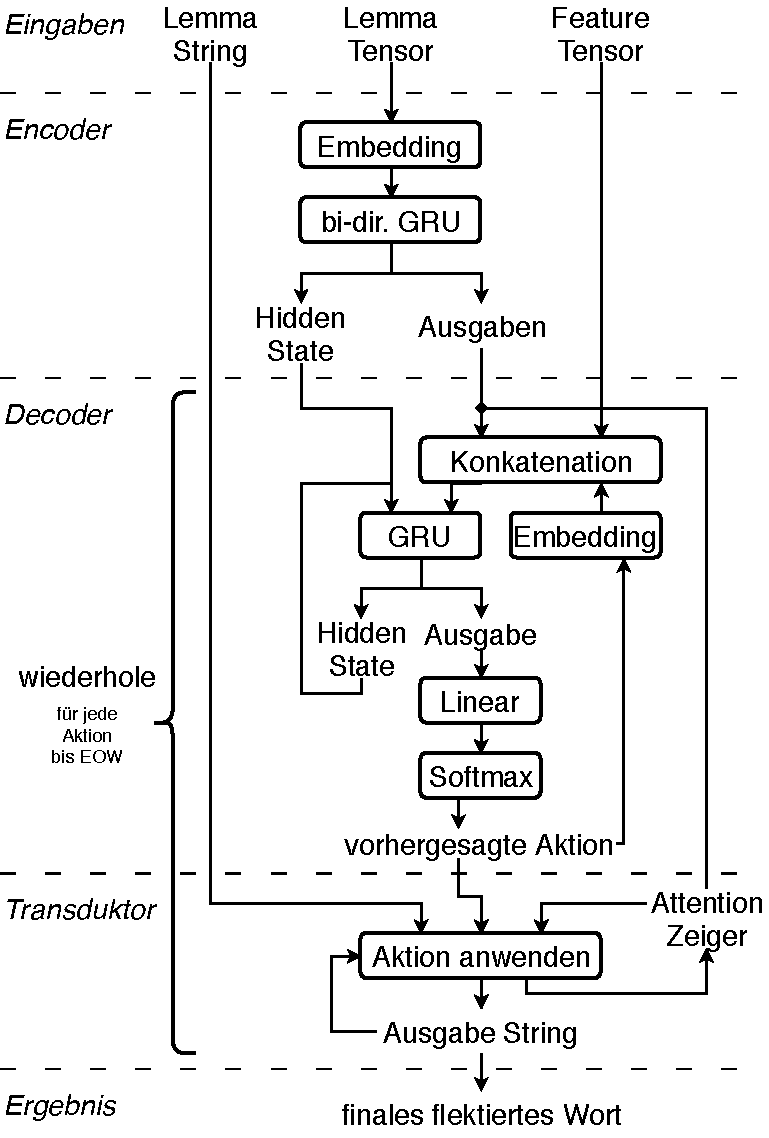
\includegraphics[width=\linewidth]{architecture_de}
\caption{System-Architektur}
\label{fig:arch}
\end{figure}
Die eingesetzte neuronale Netzwerkarchitektur unseres Systems ist für jede der 103 Sprachen und die 3 Trainingsdatenmengen identisch.
Die Architektur des Systems ist in \autoref{fig:arch} dargestellt. Das neuronale Netzwerk agiert dabei als Orakel für den String-Transduktor aus \autoref{sec:transducer}.
Eingaben des gesamten Systems sind das Lemma eines Wortes sowie die Features der Zielflektionsform.
In Abhängigkeit von Lemma, Features, aktueller Position des Zeigers und voriger Vorhersage gibt das Netzwerk je eine Aktion (\action{COPY}, \action{PATCH} $p$, \action{MOVE}, \action{EMIT} $s$ oder \action{EOW}) aus, die der String-Transduktor anwendet.
Das Vorhersagen und Anwenden einer Aktion findet für jedes Eingabewort solange statt, bis \action{EOW} durch das neuronale Netzwerk ausgegeben wird. Abschließend finalisiert der String-Transduktor die Flexion des Wortes und gibt sie aus.

In dem neuronalen Netzwerk verwenden wir eine Encoder-Decoder Architektur \citep{encdec:ChoMGBSB14, seq2seq:SutskeverVL14}, wie sie üblich ist um eine Sequenz in eine andere Sequenz zu überführen.
Maschinelle Übersetzung stellt eine der wohl geläufigsten Anwendungsfälle dieser Architektur dar.
Der Decoder wendet sich monoton den einzelnen Zeichenrepräsentationen des Lemmas zu, da sich dies für Aufgabe der morphologischen Flexion als vorteilhaft herausgestellt hat \citep{hardattention:AharoniG16,hardattention:AharoniEtAl}.
Zusätzlich ermöglicht dieses Vorgehen unserem System die \action{COPY} und \action{PATCH} Operationen sinnvoll anzuwenden, da zu jeden Zeitpunkt klar ist, welche Eingabezeichen kopiert bzw. gepatcht werden soll.

Sowohl der Encoder als auch der Decoder bestehen im Kern aus einer einzelnen Gated Recurrent Unit (GRU), die von \citet{encdec:ChoMGBSB14} als einfachere Alternative zu Long short-term memory (LSTM) entwickelt wurden.
Für jedes Zeichen erstellen Embedding-Einheiten numerische Repräsentationen als Eingabe für die beiden GRUs.
Der Encoder verwendet eine bidirektionale GRU, deren Ausgaben aus beiden Richtingen aufsummiert werden, damit auf beide Informationen auf einmal zugegriffen werden kann.
Da der Decoder unidirektional ist, verwenden wir nur den Vorwärtsweg des Encoder-Zustands um den Decoder zu initialisieren.
Im Decoder werden die Zeichen-Embeddings, der betrachtete Kontext und die Feature als Tensoren konkateniert und diese Kombination als Eingabe für die GRU genutzt.
Die Ausgabe der GRU im Decoder durchläuft eine lineare Transformation gefolgt von einer logarithmischen Softmax-Operation, um die logarithmischen Wahrscheinlichkeiten für jede Transduktor Aktion zu ermitteln. 


Bias und Gewichte für die GRUs und lineare Transformation sind zufällig anhand einer uniformen Verteilung $\mathcal{U}(-\sqrt{1/s}, \sqrt{1/s})$ initialisiert. Dabei ist $s$ die Größe des internen Zustands einer GRU bzw. die Anzahl der Eingabe-Features. Die Embedding-Gewichte sind anhand einer Normalverteilung $\mathcal{N}(0, 1)$ zufällig initialisiert.


Für die Verarbeitung eines Wortes, also Training oder Vorhersage, werden die nachfolgenden Schritte durchgeführt.
Der Encoder verarbeitet das ganze Eingabe-Lemma als indexbasierten Tensor auf einmal. Dabei generiert dieser Ausgabe-Repräsentationen für jeden Eingabe-Buchstaben  sowie eine Repräsentation des internen Zustands für die gesamte Eingabe-Sequenz.
Durch Verwendung einer externen Schleife produziert der Decoder eine einzelne Transduktor Aktion pro Schleifendurchlauf.
In jedem Schritt erhält der Decoder als Eingabe seinen vorherigen internen Zustand, die zuletzt ausgegebene Aktion, die Ziel-Flexion Features und den zurzeit betrachteten Teil der Encoder-Ausgabe.
Auf welchen Teil der Encoder-Ausgabe Zugriff gewährt wird, bestimmt der Index-Zeiger im Transduktor.
Immer, wenn der Decoder eine \action{MOVE} Aktion ausgibt, wird der Index-Zeiger um eins erhöht, sodass der Decoder im folgenden Schleifendurchlauf die Encoder-Ausgabe für das nächste Lemma-Zeichen zugreift.
Falls Aktionen den Index-Zeiger über die Länge des Lemmas hinaus schieben würden, so werde diese ignoriert.

\subsection{Beamsearch}

% dreht die Seite nicht, sondern nur die Grafik (leichter Druck, schlecht am Bildschirm)
%\begin{sidewaysfigure}[htbp]
%\centering
%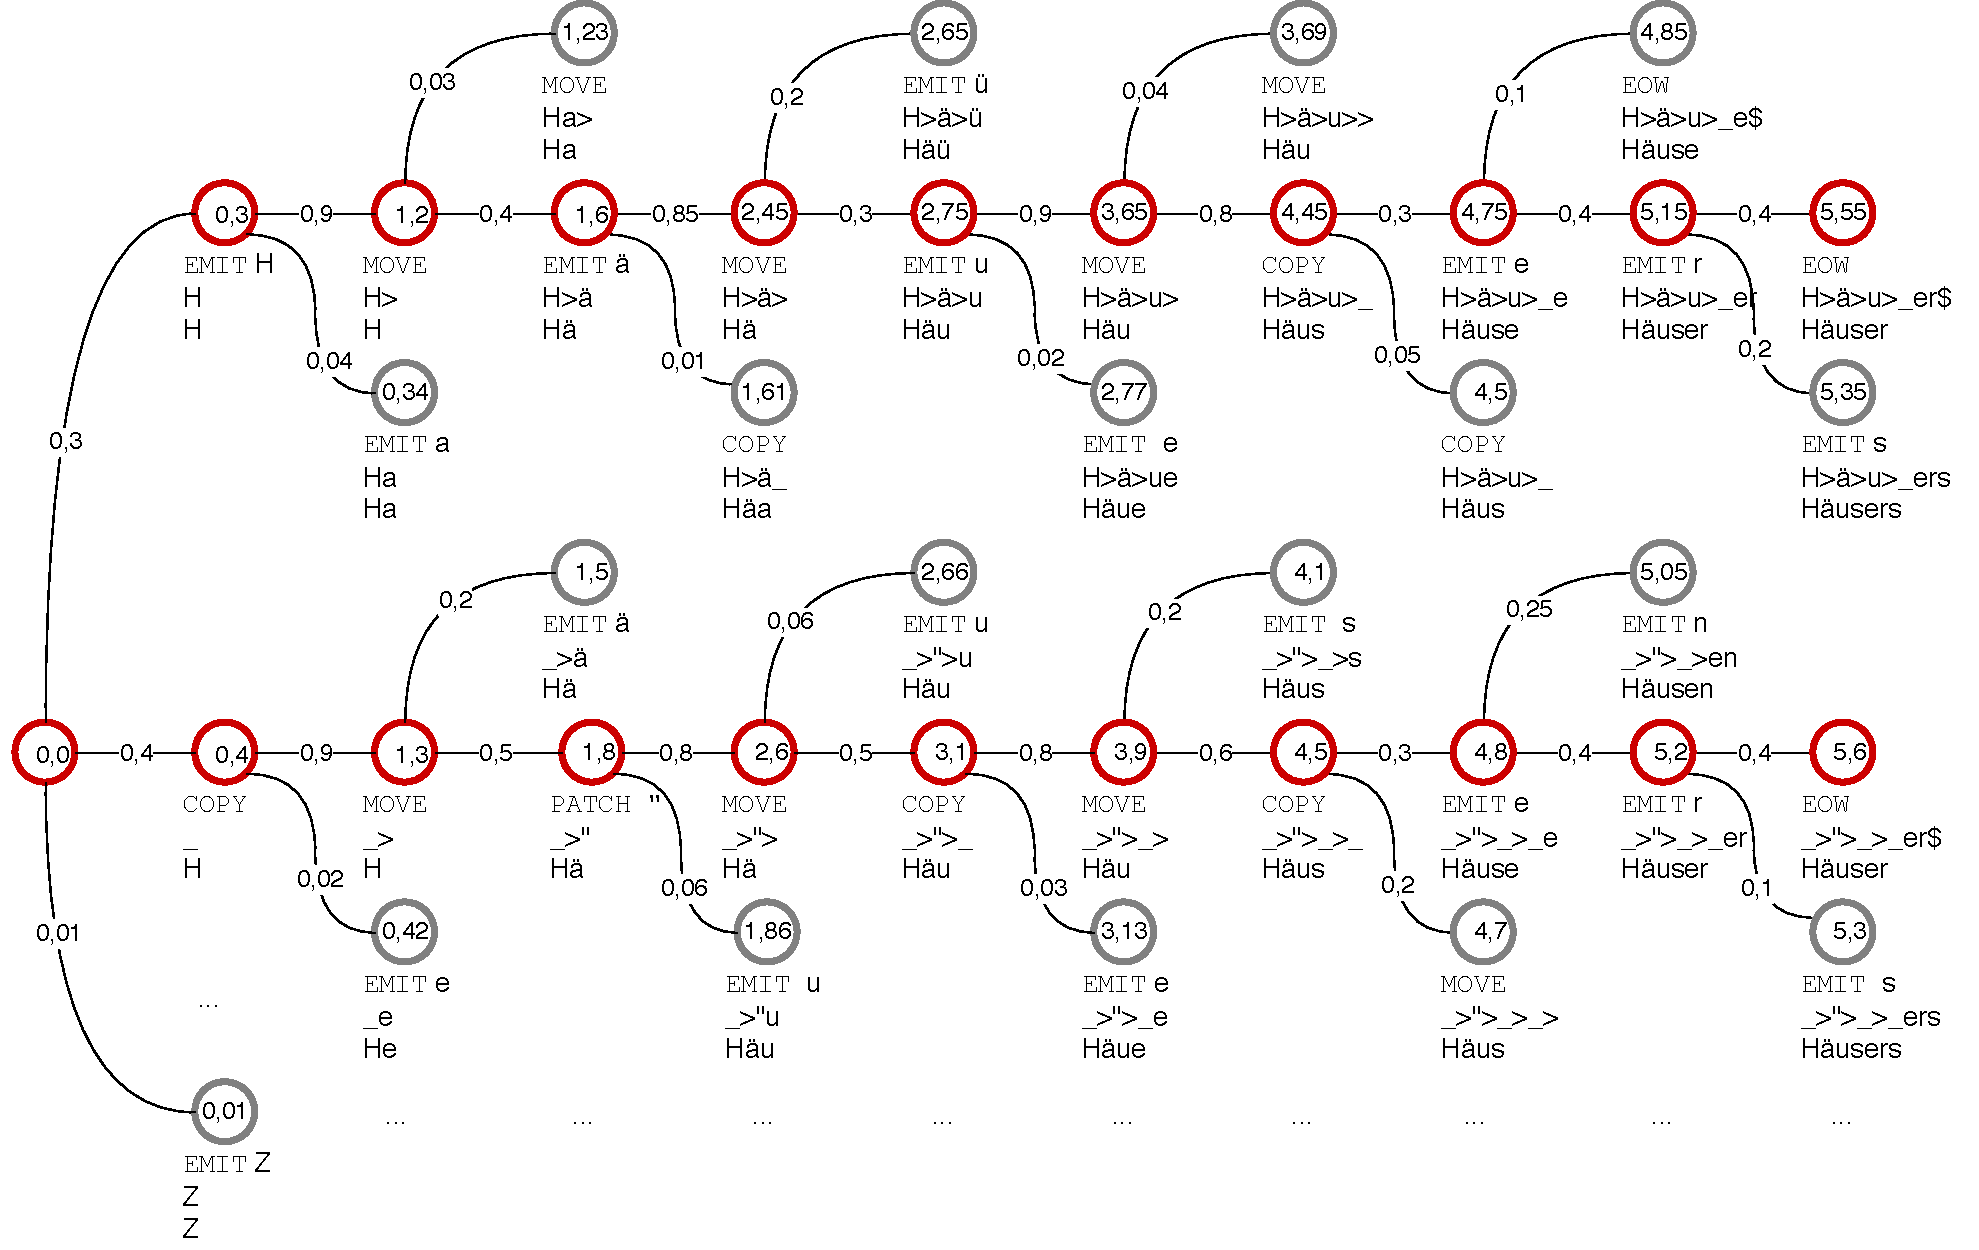
\includegraphics[width=\linewidth, height=\textheight,keepaspectratio]{beam_search}
%    \caption{Beispielhafter Beamsearch Decoding-Prozess}
%    \label{fig:beam}
%\end{sidewaysfigure}

% dreht eine ganze Seite
%\afterpage{
%\begin{landscape}
%  \begin{figure}[htbp]
%  \centering
%    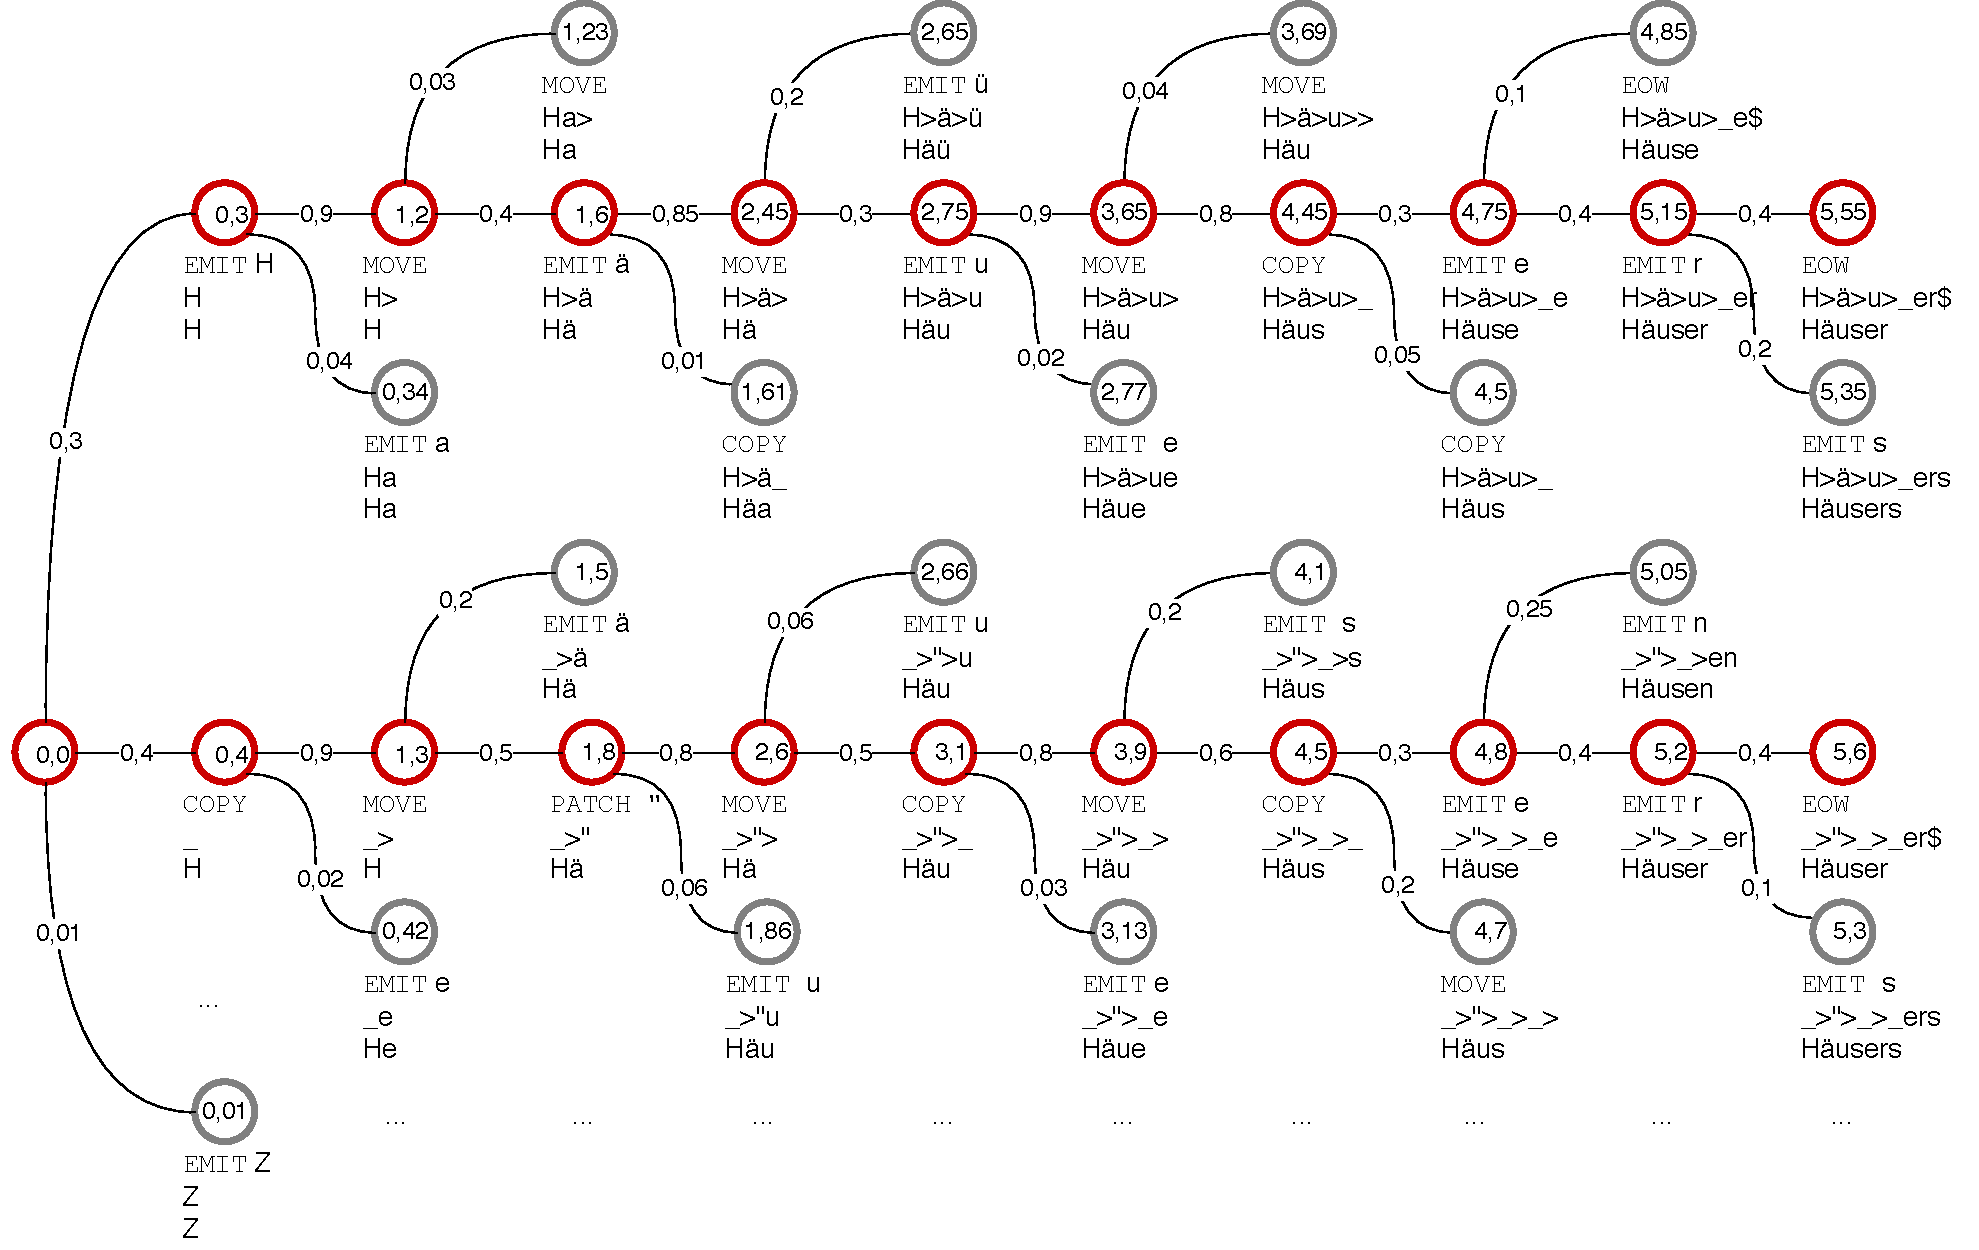
\includegraphics[width=\linewidth, height=\textheight,keepaspectratio]{beam_search}
%    \caption{Beispielhafter Beamsearch Decoding-Prozess von Haus zu Häuser mit Beam-Anzahl 2}
%    \label{fig:beam}
%  \end{figure}
%\end{landscape}
%}
\begin{sidewaysfigure*}[htbp]
  \centering
  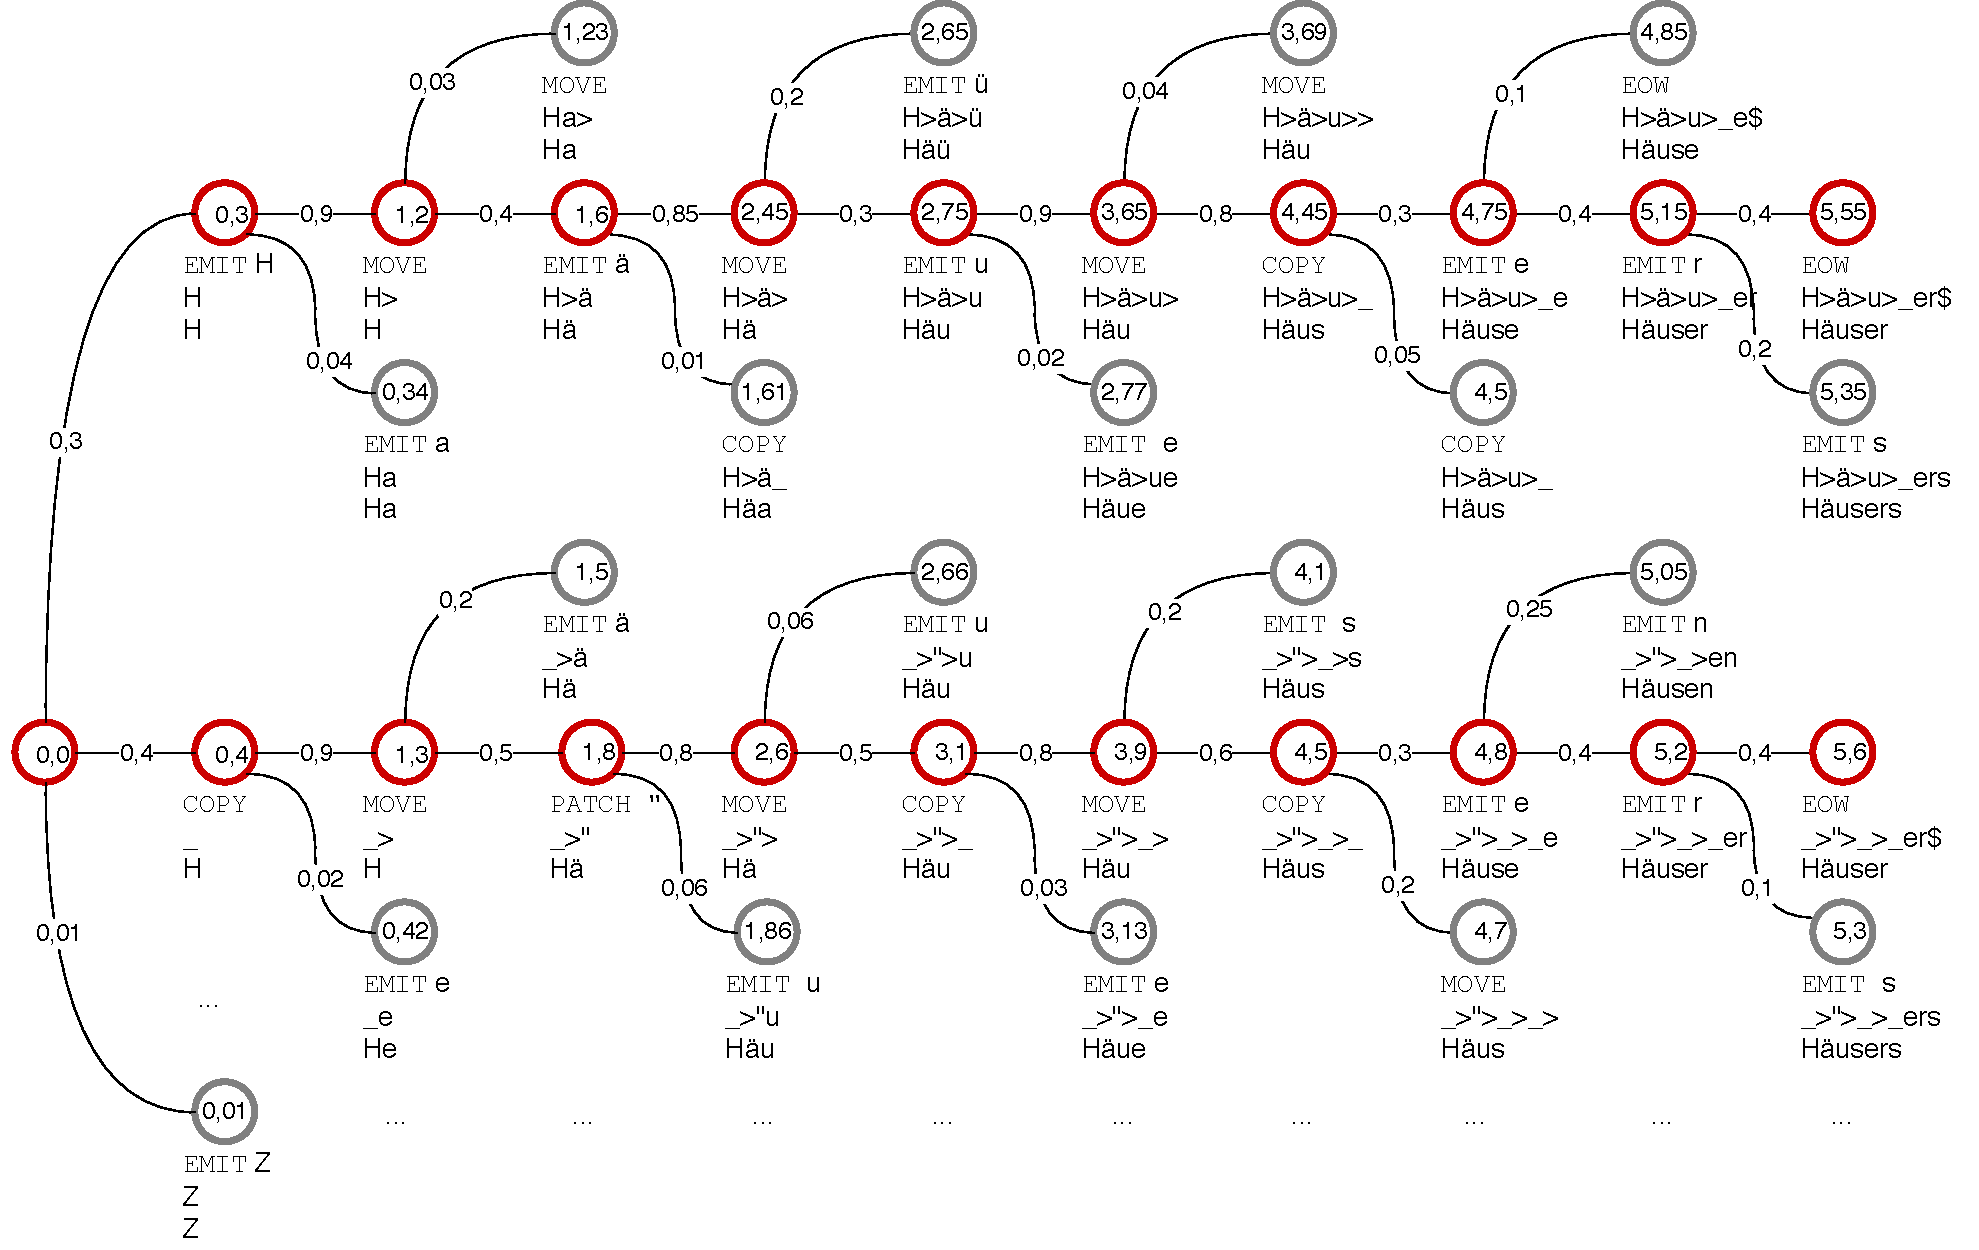
\includegraphics[width=\textwidth-\baselineskip-\abovecaptionskip-\belowcaptionskip,keepaspectratio]{beam_search}
  \caption{Beispielhafter Beamsearch Decoding-Prozess von Haus zu Häuser mit Beam-Anzahl 2}
  \label{fig:beam}
\end{sidewaysfigure*}

Um die Vorhersagegenauigkeit unseres Systems zu verbessern, haben wir Beamsearch in den Decoding-Prozess eingebaut.
Dies resultiert in mehreren Pfaden, von denen der Pfad mit der größten Wahrscheinlichkeit ausgewählt wird, um das finale flektierte Ausgabewort zu erstellen.
Die dazu benötigten Informationen werden in einem zusätzlichen Transduktorzustandobjekt vorgehalten.
Dies umfasst den internen Zustand des Decoders, die vorhergesagte Aktion mitsamt ihrer logarithmischen Wahrscheinlichkeit sowie den resultierenden Ausgabe-String für jeden Einzelschritt und Pfad im Decoding-Beam.

\autoref{fig:beam} zeigt einige Pfade eines beispielhaften Decoding-Prozesses, in dem das Lemma \texttt{Haus} in die plural Form \texttt{Häuser} überführt werden soll.
Die Kreise stellen einzelne Zustände für jeden Zeitschritt dar.
Die Zahl im inneren ist die logarithmische Wahrscheinlichkeit des Zustands, die entlang der Pfade von links nach rechts aufsummiert wird.
Das Beispiel zeigt einen Decoding-Prozess mit einer Beam-Anzahl von zwei.
Die aktiven Pfade sind durch rote Kreise markiert.
Die Zahl an der Verbindung zwischen zwei Zuständen gibt die logarithmische Wahrscheinlichkeit für die Aktion, die in der erste Zeile unterhalb eines Kreises steht, des nachfolgenden Zustands an.
In den Zeilen darunter ist die aktuelle Aktionssequenz sowie das Ergebnis der Anwendung auf das Lemma darstellt.
Für die Aktionssequenz gelten folgende Abkürzungen: \texttt{\_} entspricht \action{COPY}, \texttt{>} ist \action{MOVE}, \texttt{\"} ist die \action{PATCH} Aktion mit Umlaut und Buchstaben gelten als \action{EMIT} des jeweiligen Zeichens.

Der Decoding-Prozess in \autoref{fig:beam} startet in einem initialen Startzustand mit log. Wahrscheinlichkeit von $0$.
Das neuronale Netzwerk gibt für jede mögliche Aktion die log. Wahrscheinlichkeit an, wobei \action{COPY} in diesem Fall die höchste Wahrscheinlichkeit hat.
Da zwei aktive Pfade verfolgt werden, ist auch der Zustand der zweitwahrscheinlichsten Aktion \action{EMIT H} aktiv.
In jedem Zeitschritt wird nun für jeden aktiven, aktuellen Zustand die möglichen nächsten Zustände mit ihren Wahrscheinlichkeiten berechnet.
Aus der Gesamtmenge der neuen Zustände in diesem Zeitschritt werden dann die zwei (maximale Beam-Anzahl) mit der höchsten Wahrscheinlichkeit ausgewählt, die übrigen verworfen.
Dadurch bilden sich Pfade mit diversen abgebrochenen Abzweigungen heraus, die die höchste aufsummierte log. Wahrscheinlichkeit innehaben.
Dieses Vorgehen wird solange fortgesetzt bis zwei Pfade zum Ende (Aktion \action{EOW}) gelangen.
Aus diesen wird nun der beste Pfad (mit höchster log. Wahrscheinlichkeit) ausgewählt, um die finale Ausgabe der Flexion zu erstellen.
In diesem Fall ist dies der untere rote Pfad, welcher \texttt{Haus} nach \texttt{Häuser} mittels der Aktionskette \action{COPY} \action{MOVE} \action{PATCH "} \action{MOVE} \action{COPY} \action{MOVE} \action{COPY} \action{EMIT e} \action{EMIT r} transformiert.

Der große Vorteil des Beam-Decodings liegt darin bessere Lösungen als das gierige Dekodieren (\textit{greedy decoding}) zu finden, indem mehrere Pfade weiterverfolgt werden.
Wenn Pfad mit der zuerst höchsten Wahrscheinlichkeit sich später als absolut unbrauchbar heraus stellt, treten im Beam-Decoding andere Pfade an seine Stelle und führen so zu einem meist besseren Ergebnis.
Die Auswirkungen von Beam-Decoding auf die Ergebnisse unseres Systems werden in \autoref{sec:beam-results} vorgestellt.

Für die Verbesserung der Vorhersage mittels Beam-Decoding wird allerdings auch eine erhöhte Rechenleistung erfordert.
Der Aufwand des Decoders steigt in etwa linear mit der Beam-Anzahl an. 
Diese Kosten sind jedoch nur in der finalen Evaluation zu zahlen, da während des Trainings kein Beam-Decoding stattfinden muss.
Es kann jedoch auch dazu verwendet werden, das Training des Netzwerkes zu verbessern wie in \autoref{sec:training} erläutert wird.


\subsection{Training}
\label{sec:training}
Da das neuronale Netzwerk eine Sequenz von Transduktor Aktionen ausgibt, handelt es sich bei den Trainingszielen nicht um flektierte Wörter, sondern ebenfalls um Aktionssequenzen, die die eigentlichen Flexionen produzieren, wenn sie auf das Lemma angewandt werden.
Diese Aktionssequenzen werden zuvor von unserem System erzeugt, indem im Gleichschritt über das alignierte Lemma und das flektierte Wort iteriert wird.
Für jede Zeichenkombination werden die zugehörigen Aktionen der neuen Ausgabesequenz hinzugefügt.
Der Algorithmus ist im Detail in \autoref{sec:orakel-alg} beschrieben.


Trainingsupdates werden mittels Backpropagation durch den Adam Optimierer \citep{adam:KingmaB14} durchgeführt.
Dieser ist mit den folgenden Paramtern konfiguriert: \textit{Learning rate} $\alpha=0.005$, \textit{Momentum Decays} $\beta_1=0.9$, $\beta_2=0.999$, \textit{Numerical Stabilizer} $\epsilon=10^{-8}$ und \textit{Weight Decay} (L2 Regularisierung) von $0.001$.


Das implementierte Beam-Decoding erlaubt eine globale Normalisierung des neuronalen Netzwerks laut \citet{globalnorm:AndorAWSPGPC16}.
Leider konvergiert das Training des Models mit globaler Normalisierung und Beamsearch in unseren Versuchen nicht.
\citet{globalnorm:AndorAWSPGPC16} haben vortrainierte Gewichte mittels lokaler Normalisierung verwendet, um dieses Problem zu umgehen.
Da wir allerdings keine robuste Möglichkeit zum Wechseln von lokaler zu globaler Normalisierung für alle 103 Sprachen finden konnten, setzen wir ausschließlich lokale Normalisierung im Training ein.
Sobald der korrekte Pfad aus dem Beam während des Dekodierens fällt, wird ein Trainingsupdate mit unserer spezifischen \textit{Loss}-Funktion auf Grundlage der logarithmischen Wahrscheinlichkeiten der einzelnen Schritte im korrekten Pfad durchgeführt.


Die \textit{Loss}-Funktion in \autoref{eq:loss} basiert auf der lokal normalisierten Pfadwahrscheinlichkeit, die als Gleichung (4) in \citet{globalnorm:AndorAWSPGPC16} dargestellt ist.
Sie berechnet die negierte Summe über die logarithmischen Wahrscheinlichkeiten $l$ der korrekten Aktion für jeden Schritt des Pfades.
Das Dividieren durch den natürlichen Logarithmus der Sequenzlänge $s$ führt zu gleichmäßigeren \textit{Loss}-Größenordnungen, was dem Trainingsprozess hilft besser zu konvergieren.
Wir vermuten, dass dies der Fall ist, da wir die Fehler über alle Schritte aufsummieren, wozu auch korrekte Vorhersagen zählen bei denen das System nur nicht 100 \% sicher ist.
Das berechnete Ergebnis $L$ der Funktion wird anschließend verwendet, um die Trainingsupdates mittels \textit{Backpropagation} zurück durch das gesamte neuronale Netzwerk durchzuführen.


\begin{equation}
\label{eq:loss}
L = - \frac{\sum_i^s l_i}{\ln{(1+s)}}
\end{equation}


Durch den Verzicht auf globale Normalisierung und die Verwendung von lokaler Normalisierung konnten wir das Konvergieren des Lernprozesses wiederherstellen. Allerdings konnten wir dadurch keine signifikanten Vorteile in der Verwendung mehrerer Beams während es Trainings finden.
Eine mögliche Erklärung weshalb unser Netzwerkmodell im Training nicht von Beam-Decoding profitiert ist, dass das Modell viele Trainingsupdates erfordert.
Während durch das Bestrafen korrekter Schritte des Decoding-Prozesses viele Trainingsupdates entstehen, könnten diese bei Beam-Decoding zu selten sein, da mit höherer Wahrscheinlichkeit ein korrekter Pfad im Beam vorhanden ist.


Zur Abgabe der Daten für den Shared Task haben wir auf Beam-Decoding verzichtet, indem wir als Anzahl der Pfade $1$ verwendet haben.
Die entwickelte Architektur ist allerdings bereit sowohl Beam-Decoding als auch globale Normalisierung zu verwenden.
Auf dieser Grundlage haben wir auch noch weitere Untersuchungen vorgenommen, die später vorgestellt werden.
So ist beispielsweise auch das Trainieren mit einem einzigen Pfad und gleichzeitiges Evaluieren mit mehreren Pfaden möglich. Dadurch kann die Vorhersage verbessert werden, ohne die Trainingslaufzeit zu erhöhen.
Aufgrund der relativ komplexen Implementierung des Beam-Decoding haben wir bis zur Abgabe des Shared Tasks kein Mini-Batching implementiert. Nachträglich ist jedoch auch Mini-Batching eingebaut worden, um das Training hinsichtlich Konvergenz und Rechner-Ressourcenauslastung zu optimieren.

\section{Feinabstimmung und Evaluation}
\label{sec:tuning_evaluation}

\begin{table*}[htb]
    \centering
    \begin{tabularx}{\textwidth}{lcX}
    \toprule
    Parameter & Werte & Beschreibung\\
    \midrule
        GRU Größe & 32, 64, 128 & Tensor Größe des internen Zustands von Encoder \& Decoder\\
        Embedding Größe & 8, 16 & Tensor Größe der Zeichen-Embeddings\\
        Patches & ja, nein & Verwendung der Patches aktiv?\\
        Enhancer & 0\times, 1\times, 5\times & Faktor der Erzeugung zusätzlicher Trainingsdaten\\
    \bottomrule
    \end{tabularx}
    \caption{Hyperparameter}
    \label{tab:params}
\end{table*}

Um die Ergebnisse unseres Systems zu verbessern, haben wir eine extensive Hyperparameter-Suche vorgenommen.
Der zuvor geschilderte Aufbau des Systems ist dabei für alle Sprachen identisch.
Je Sprache und Größe des Trainingsdatensatzes haben wir eine unabhängige Hyperparameter-Suche auf einer zufälligen Auswahl aus dem Such-Raster der Parameter durchgeführt.
\autoref{tab:params} listet die Hyperparameter mitsamt ihrer möglichen Werte auf.

Während der Entwicklungsphase des Systems ist uns aufgefallen, dass die zufällige Initialisierung der Netzwerkgewichte großen Einfluss auf die Ergebnisse haben. Es handelt sich dabei um ein typisches Problem, welches insbesondere dann auftritt, wenn nur wenige Traningsdaten zur Verfügung stehen.
Aus diesem Grund wird in unserer Hyperparamter-Suche jede Parameterkombination mit fünf verschiedenen Zufalls-Seeds durchlaufen, wodurch sowohl die Netzwerkgewichte andere Startwerte annehmen als auch die Reihenfolge der einzelnen Trainingsdatenpunkte variiert.

Die Hyperparameter-Suche erstreckt sich insgesamt über 103 Sprachen, 3 Trainingsdatensätze, 3 GRU Größen, 2 Embedding Größen, 2 Patch-Zustände, 3 Enhancer-Stufen und 5 Zufalls-Seeds, was in $103 \times 3 \times 3 \times 2 \times 2 \times 3 \times 5 = 55.620$ Parameterkombinationen resultiert.
Jeder einzelne Durchlauf erfordert ein vollständiges Training des neuronalen Netzwerkes sowie die Erzeugung der Ausgabedaten.
Dies dauert in etwa ein bis drei Minuten für den kleinsten, zehn bis 20 Minuten für den mittleren und ein bis zwei Stunden für den größten Trainingsdatensatz.

Da eine erschöpfende Suche von $55.620$ Parameterkombinationen zu viel Rechenzeit in Anspruch nähme, haben wir Möglichkeiten erkundet um die Anzahl zu reduzieren. Für den mittleren Trainingsdatensatz werden nur GRU und Embedding Größen getestet, die größer oder gleich dem besten Ergebnis auf dem kleinen Trainingsdatensatz sind.
Analog dazu ist der große Datensatz ebenfalls in diesen beiden Parametern durch die besten Ergebnisse des mittleren Datensatzes beschränkt.
Dies ist naheliegend, da mit steigenden Anzahl von Gewichten im neuronalen Netzwerk mehr Trainingsdaten benötigt werden, damit kein \textit{Overfitting} eintritt.
Zusätzlich verwenden wir den Enhancer ausschließlich auf dem kleinen Trainingsdatensatz, da bereits das mittlere genügend Traningsexemplare enthält.
Aus diesen reduzierten Parameterkombinationen wird je Sprache und Größe der Trainingsdaten eine zufällige Auswahl gezogen, um eine feste obere Grenze an Trainingsdurchläufen zu garantieren.
Für die Abgabe der Ergebnisse für den Shared Task hat unsere Hyperparameter-Suche $9.278$ Trainingsläufe durchgeführt, was fast einer Reduktion auf ein Sechstel der ursprünglichen Menge entspricht.

Während einer frühen Evaluation der Ergebnisse konnten wir feststellen, dass unser System in der Vorhersage manchmal das Wort nicht mit \action{EOW} beendet und stattdessen endlos einen nicht existierenden Buchstaben des Lemmas mit \action{COPY} kopieren möchte oder aber ein beliebiges Zeichen mit \action{EMIT} andauernd wiederholt.
Daher enthält der String-Transduktor Maßnahmen um diese Probleme zu entschärfen.
Wenn der Zeiger bereits über das Eingabewort hinaus bewegt wurde, greifen folgende Regelungen:
Die Aktionen \action{COPY} und \action{PATCH} werden nicht mehr angewandt. Die \action{EMIT} Aktion kann das zuvor geschriebene Zeichen nicht erneut ausgeben. 
Dadurch können jedoch die flektierten Formen in einigen Ausnahmefällen einzelne Zeichen am Ende vermissen. 

Für die finale Evaluation der Testdatensätze haben wir die beste Parameterkombination (inklusive Zufalls-Seed) für ein jedes Paar aus Sprache und Größe des Trainingsdatensatzes auf Basis der Levenshtein-Distanz der Ergebnisse auf dem bereitgestellten Entwicklungsdatensatz verwendet.


\section{Ergebnisse und Diskussion}
\label{sec:results}

\subsection{Eingereichte Ergebnisse}
\label{sec:eingereichte_ergebnisse}

\begin{table*}[tbh]
%\small
\centering
\begin{tabular}{lr|lr|lr}
\toprule
\textbf{high}             & & \textbf{medium}                 &  & \textbf{low}                  &  \\
\midrule
Teilnehmer                 & Accuracy                    & Teilnehmer                & Accuracy                      & Teilnehmer                & Accuracy
\\
\rule{0pt}{3ex}uzh-01                     & 96                     & uzh-01                     & 86.64                   & uzh-02                     & 57.21                  \\
uzh-02                     & 95.97                  & uzh-02                     & 86.38                   & uzh-01                     & 57.18                  \\
bme-02                     & 94.66                  & iitbhu-iiith-02            & 84.19                   & ua-08                      & 53.22                  \\
iitbhu-iiith-02            & 94.43                  & iitbhu-iiith-01            & 82.9                    & iitbhu-iiith-02            & 52.6                   \\
iitbhu-iiith-01            & 94.43                  & waseda-01                  & 77.38                   & ua-05                      & 50.53                  \\
bme-03                     & 93.97                  & msu-04                     & 76.4                    & iitbhu-iiith-01            & 49.79                  \\
bme-01                     & 93.88                  & msu-03                     & 75.74                   & ua-06                      & 49.73                  \\
msu-04                     & 91.87                  & \textbf{hamburg-01}        & \textbf{74.03}          & ua-03                      & 44.82                  \\
iit-varanasi-01            & 91.73                  & iit-varanasi-01            & 70.17                   & waseda-01                  & 44.09                  \\
waseda-01                  & 91.12                  & msu-02                     & 69.45                   & msu-02                     & 41.61                  \\
msu-03                     & 90.52                  & bme-01                     & 67.43                   & \textbf{hamburg-01}        & \textbf{40.28}         \\
axsemantics-01             & 84.19                  & bme-03                     & 67.36                   & ua-02                      & 39.19                  \\
msu-02                     & 82.68                  & bme-02                     & 67.26                   & ua-01                      & 38.22                  \\
\textbf{hamburg-01}        & \textbf{77.53}         & \textit{\textbf{baseline}} & \textit{\textbf{61.78}} & \textit{\textbf{baseline}} & \textit{\textbf{38.2}} \\
\textit{\textbf{baseline}} & \textit{\textbf{75.3}} & axsemantics-02             & 60                      & ua-07                      & 37.99                  \\
axsemantics-02             & 74.77                  & msu-01                     & 54.44                   & msu-04                     & 31.4                   \\
msu-01                     & 74.33                  & tuebingen-oslo-03          & 30.98                   & msu-03                     & 25.86                  \\
racai-01                   & 72.49                  & tuebingen-oslo-02          & 29.72                   & iit-varanasi-01            & 23.33                  \\
tuebingen-oslo-03          & 63.05                  & kucst-01                   & 29.12                   & ua-04                      & 21.25                  \\
tuebingen-oslo-02          & 56.6                   & tuebingen-oslo-01          & 20.97                   & axsemantics-02             & 14.74                  \\
tuebingen-oslo-01          & 49.52                  & axsemantics-01             & 9.1                     & tuebingen-oslo-02          & 4.43                   \\
kucst-01                   & 48.68                  & ua-08                      & 0                       & bme-01                     & 3.74                   \\
ua-08                      & 0                      & ua-07                      & 0                       & bme-03                     & 3.63                   \\
ua-07                      & 0                      & ua-06                      & 0                       & kucst-01                   & 2.52                   \\
ua-06                      & 0                      & ua-05                      & 0                       & bme-02                     & 2.43                   \\
ua-05                      & 0                      & ua-04                      & 0                       & tuebingen-oslo-03          & 1.39                   \\
ua-04                      & 0                      & ua-03                      & 0                       & axsemantics-01             & 0.7                    \\
ua-03                      & 0                      & ua-02                      & 0                       & tuebingen-oslo-01          & 0                      \\
ua-02                      & 0                      & ua-01                      & 0                       & racai-01                   & 0                      \\
ua-01                      & 0                      & racai-01                   & 0                       & msu-01                     & 0         
\\
\bottomrule
\multicolumn{6}{l}{$0$: keine Einreichung des Teilnehmers}
\end{tabular}

\caption{Ergebnisse (Accuracy) aller Teilnehmer am Shared Task für alle Mengen.}
%Abrufbar unter: \url{https://docs.google.com/spreadsheets/d/1HqOGRyltYvji7pi-jq3swEfoWs15k5QU-lA3ua8dpmo/}
\label{fig:results_all}
\end{table*}

\begin{table}
\centering
\begin{tabular}{lrrr}
\toprule
                 & high   & medium & low    \\
                 \midrule
Baseline         & 75.5\% & 64.8\% & 38.2\% \\
Ø aller Systeme & 81.3\% & 61,0\% & 30.7\% \\
Wir              & 77.5\% & 74,0\% & 40.3\% \\
\bottomrule
\end{tabular}
\caption{Unsere Ergebnisse (Accuracy) im Vergleich.  Durchschnitt ohne $0$}
\label{fig:acc_comparison}
\end{table}

\begin{table}
\centering
\begin{tabular}{lrrr}
\toprule
         & high & medium & low  \\
         \midrule
Baseline & 0.52 & 0.91   & 1.86 \\
Wir      & 0.45 & 0.52   & 1.47\\
\bottomrule
\end{tabular}
\caption{Unsere Ergebnisse (durchschnittliche Levenshtein-Distanz) im Vergleich zur Baseline. Levenshtein-Ergebnisse anderer Teilnehmer lagen nicht vor.}
\label{fig:lev_comparison}
\end{table}

In \autoref{fig:results_all} sind die veröffentlichten Ergebnisse aller Teilnehmer für alle Datenmengen dargestellt. Wir konnten uns im guten Mittelfeld positionieren und stets die Baseline schlagen.

Die beste Position (Position 8 von 21, oberen $38.1\%$) und die größte Verbesserung im Vergleich zur Baseline ($+12.15\%$) konnten wir mit einer Genauigkeit von $74.03\%$ auf der Menge \textit{medium} erreichen . Auf \textit{high} und \textit{low} lagen unsere Ergebnisse mit $77.53\%$ bzw. $40.28\%$ etwa $2\%$ über der Baseline und in den oberen $63.6\%$ beziehungsweise $40.7\%$ der eingereichten Ergebnisse.

In Tabellen \ref{fig:acc_comparison} und \ref{fig:lev_comparison} sind unsere Ergebnisse nach Accuracy und Levenshtein im Vergleich zur Baseline sowie zum Durchschnitt der anderen Teilnehmern (nur Accuracy) aufgeführt. Wir konnten die durchschnittliche Accuracy der Teilnehmer auf \textit{medium} ($+13.0\%$) und \textit{low} ($+9.6\%$) schlagen. Die durchschnittliche Levenshtein-Distanz der Baseline konnten wir auf allen Mengen schlagen. Besonders auf \textit{medium} ($-0.39$) ist die Verbesserung mit $42.9\%$ deutlich, bei \textit{high} ($-0.07$, Verbesserung um $13.5\%$) und \textit{low} ($-0.39$, Verbesserung um $21.0\%$) weniger deutlich.

\autoref{tab:langs_baseline} zeigt die Sprachen, die am Weitesten \textbf{über} und \textbf{unter} der Baseline lagen. In \autoref{sec:schwachstellen} werden die Schwachstellen des Systems beschrieben, die mit hoher Wahrscheinlichkeit zumindest zum Teil für die schlechten Ergebnisse auf manchen Sprachen verantwortlich sind.

\begin{table}
\centering
\small
\begin{tabular}{llrr}
  \toprule
                           & \textbf{Sprachen}  &\textbf{Wir} & \textbf{BL} \\
\midrule\textbf{Beste}   & Uzbek              & $100.0$      & $96.0$ \\
                           & Mapudungun         & $100.0$      & $82.0$ \\
                           & Classical-Syriac   & $97.0$       & $99.0$ \\
%\midrule
\textbf{Schlechteste}         & Old-Irish          & $6.0$        & $16.0$ \\
                           & Haida              & $16.1$       & $61.0$ \\
                           & Latin              & $21.4$       & $37.6$ \\
%\midrule
\midrule
\textbf{max(Wir - BL)}    & Swahili            & $95.0$         & $0.0$ \\
                           & Murrinhpatha       & $88.0$       & $0.0$ \\
                           & Zulu               & $81.8$       & $0.1$ \\
\textbf{max(BL - Wir)}    & Neapolitan         & $49.0$       & $94.0$ \\
                           & Haida              & $16.0$       & $61.0$ \\
                           & Latin              & $21.4$       & $37.6$ \\
\bottomrule
\end{tabular}

\vspace{1ex}
\textbf{Über Baseline:} $73$  \quad \textbf{durchschn. Diff.:} $20.2$\\
\textbf{Unter Baseline:} $29$ \quad \textbf{durchschn. Diff.:} $-7.7$
\caption{Unsere Ergebnisse verglichen mit der Baseline. Sprachen am weitesten \textbf{über} und \textbf{unter} der Baseline, trainiert auf dem Training-Set \textit{medium} und evaluiert auf dem Test-Set.}
\label{tab:langs_baseline}
\end{table}


\subsection{Effekt von Patches und Enhancer}
\todo[inline]{Effekt von Patches}

Auf die niedrige Datenmenge verbesserte der künstlich erweiterte Datensatz (bestes Ergebnis von \times 1 und \times 5) die Accuracy von 42 Datensätzen. Die Wahrscheinlichkeit, dass dies zufällige Beobachtungen sind, liegt bei $0.3049$ \citep{biostat:zar}. Der durchschnittliche Effekt über alle Sprachen beträgt $+1.3\%$, die maximale Verbesserung konnte mit $+10.8\%$ auf \lang{french} erreicht werden.

\subsection{Effekt Beam-Decoding}
\label{sec:beam-results}

\begin{figure}
\centering
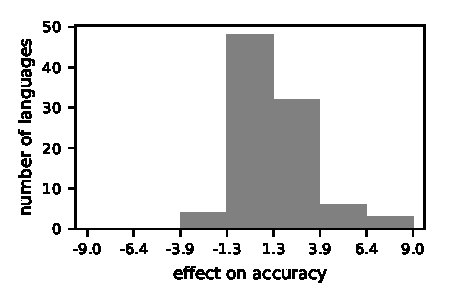
\includegraphics{beamlow}
\caption{Histogramm, welches den Effekt von Beam-Größe 16 im Vergleich zu Größe 1 auf dem Test-Datensatz zeigt (Trainiert auf dem kleinsten Datensatz)
\todo[inline]{Bild Beschriftung auf Deutsch}
}
\label{fig:histBeamLowAcc}
\end{figure}

Auch wenn wir Beam-Decoding für die Einreichung der Daten zum Shared Task nicht verwendet haben, so haben wir im Nachgang Experimente hinsichtlich der Veränderung der Evaluationsergebnisse durchgeführt.
\autoref{fig:histBeamLowAcc} zeigt für wie viele Sprachen ein Unterschied hinsichtlich der Accuracy durch Beam-Decoding mit einer Größe von 16 im Vergleich zu deaktivierten Beam-Decoding auftritt.
Knapp die Hälfte der Sprachen zeigt keine oder nur minimale Veränderungen der Accuracy durch Beam-Decoding.
Etwa ein Drittel der Sprachen weist eine leichte Verbesserung der Accuracy zwischen $1,3$ und $3,9$ auf.
Während bei einigen Sprachen sogar ein noch stärkerer Anstieg der Accuracy auftritt, zeigen nur wenige Sprachen eine minimale Verschlechterung durch Beam-Decoding.

Über alle Sprachen gemittelt führt der Einsatz von Beam-Decoding mit Größe 16 zu einer Erhöhung der Accuracy von 4\%.
% A binomial test shows that the probability of the increase being random is as low as $2.4 \times 10^{-10}$. Beam-decoding therefore clearly leads to an increase in accuracy which matches the intuition of beam-decoding producing better or equal results compared to greedy decoding.
Ein Binomialtest zur Prüfung, ob es sich ausschließlich um zufällige Erhöhungen handelt, weist im Ergebnis eine Wahrscheinlichkeit von nur $2.4 \times 10^{-10}$ auf.
Daher führt Beam-Decoding zu einem merklichen Anstieg der Accuracy, was auch mit der Intuition übereinstimmt, dass Beam-Decoding nur bessere oder gleiche Ergebnisse im Vergleich zu \textit{greedy decoding} liefert.


\subsection{Schwachstellen}
\label{sec:schwachstellen}
Unser System weist mehrere Schwachstellen auf, von denen manche bewusste Architekturentscheidungen sind, andere jedoch aus einer suboptimalen Implementierung entstanden.

% --- fehlerhafte Umsetzung
So ist die Accuracy unseres Systems bei den Sprachen \lang{Neapolitan} und \lang{Haida} deutlich schlechter im Vergleich zu anderen Systemen und der Baseline wie \autoref{tab:langs_baseline} zeigt.
Die Ursache dafür liegt in der fehlerhaften Nachverarbeitung des String-Transduktors.
Der in \autoref{sec:tuning_evaluation} beschriebene Ausnahmefall beim Korrigieren fehlender \action{EOW}-Ausgaben des neuronalen Netzwerkes tritt für die Sprachen \lang{Neapolitan} und \lang{Haida} oft irrtümlicherweise auf.
Das nachfolgende Beispiel aus dem Test-Datensatz zu \lang{Haida} zeigt, wie unser System in der Ausgabe ein Zeichen verschluckt, da der Transduktor die wiederholte \action{EMIT a} Aktion ignoriert, obwohl das neuronale Netzwerk in diesem Fall eine richtige Vorhersage gemacht hat:
\begin{compactitem}
	\item \texttt{ñíiyä} $\to$ \texttt{ñíiyä'wa\underline{\ }} (Vorhersage)
    \item \texttt{ñíiyä} $\to$ \texttt{ñíiyä'wa\underline{a}} (Ziel)
\end{compactitem}
Solche und ähnliche Fehler treten vereinzelt in den meisten Sprachen auf -- doch in \lang{Neapolitan} und \lang{Haida} sind besonders viele Flexionen betroffen.
Da sich Vorhersage und Ziel-Form jedoch meist nur um ein Zeichen unterscheiden, ist die Levenshtein-Distanz deutlich niedriger als die Accuracy auf den ersten Blick vermuten lässt.
Während bei \lang{Haida} unser System eine deutlich geringere Accuracy als die Baseline liefert, schlägt unser System die Baseline auf dem gleichen Datensatz dennoch hinsichtlich der Levenshtein-Distanz.

Die suboptimale Nachverarbeitung im Transduktor hat sich im Rückblick als sehr ärgerlicher Fehler herausgestellt.
Wäre die Nachverarbeitung wie geplant nur dann aktiv geworden, wenn das neuronale Netzwerk gar kein \action{EOW} innerhalb der zulässigen Höchstlänge ausgibt, so hätte die Accuracy unseres Systems im Einklang zu den guten Levenshtein-Ergebnissen eine merkliche Verbesserung gezeigt.

Noch besser wäre es hingegen auf die Nachverarbeitung in Gänze verzichten zu können. Eine Möglichkeit dazu ist die Verbesserung des Trainingsprozesses, indem ein dynamisches Orakel anstelle der statischen Ziel-Sequenz verwendet wird.
Zusätzlich könnte noch globale Normalisierung bein Beam-Decoding eingesetzt werden.
Die Anpassungen am Training des neuronalen Netzwerkes sollten die Probleme der bisherigen Netzwerkausgabe beheben, wodurch auf die fehlerhafte Nachverarbeitung vollständig verzichtet werden kann. 

% --- bewusste Architekturentscheidungen
Eine ganz andere Schwachstelle unseres Systems folgt aus bewusst getroffenen Architekturentscheidungen.
So fällt es unserem System äußerst schwer Präfixe in Suffixe umzuwandeln und umgekehrt. Das folgende Beispiel aus dem Datensatz für \lang{German} verdeutlicht das Problem:
\begin{compactitem}
	\item \texttt{\underline{ab}stellen} $\to$ \texttt{stellt \underline{\ \ }} (Vorhersage)
    \item \texttt{\underline{ab}stellen} $\to$ \texttt{stellt \underline{ab}} (Ziel)
\end{compactitem}
Das System ist nicht in der Lage den Präfix \texttt{ab} des Lemmas am Ende der Flexion anzufügen.
Dies ist ein zu erwartendes Verhalten, da unser System die Repräsentationen der Buchstaben in monoton nacheinander bearbeitet ohne die Möglichkeit frei auf die verschiedenen Stellen des Lemmas zuzugreifen.
Das neuronale Netzwerk müsste daher die Information des zu Beginn gelesenen Präfixes des Lemmas so lange im internen Zustand speichern bis diese am Ende der Flexion wieder ausgeben werden soll, da dem Decoder nicht gestattet ist erneut auf den Anfang des Lemmas zuzugreifen nachdem das Lemma bereits vollständig durchlaufen wurde.

Um jenes Problem zu lösen, müsste der Decoder mittels \textit{soft-attention} freien Zugriff auf die gesamte Ausgabe des Encoders erhalten. Dadurch wäre jedoch eine erfolgreiche Anwendung der \action{COPY} und \action{PATCH} Aktionen auf dem Lemma nicht mehr gegeben, was jedoch den Kern unseres Systems ausmacht.

\section{Teilnahme am Shared Task und Paper}
\label{sec:paper}
\todo{besser benennen}
\todo[inline]{Hier können wir schreiben, wie wir am Shared Task teilgenommen haben (Wann wir die Daten bekommen haben, wann wir was abgegeben haben etc.), statt es wie in der Präsentation etwas zu verteilen. Und eben über das Paper berichten. Können das aber wieder trennen oder die Teilnahme-Details ganz weglassen.}

Pünktlich zur Frist der ersten Abgabe haben wir den ersten Entwurf des Papers anonymisiert am 15. August 2018 eingereicht. Das Paper \enquote{Finding the way from ä to a: Sub-character morphological inflection for the SIGMORPHON 2018 Shared Task}\footnote{abrufbar unter \url{https://arxiv.org/abs/1809.05742}} ist acht Seiten lang plus Bibliographie. Am 23. August 2018 haben wir die Nachricht bekommen, dass das Paper akzeptiert wurde, sowie das Feedback zweier anonymer Kritiker erhalten. Dieses beinhaltete unter anderem, dass das Paper \enquote{verständlich geschrieben} sei, mehr Experimente zum Effekt der Patches nötig seien, weitere Zitate für den Enhancer sowie den Hinweis auf Unicode NDF-Dekomposition. Außerdem haben beide Gutachter das Paper nach bestimmten Kriterien bewertet, siehe Tabelle \ref{tab:review}. Beide Reviewer haben dabei die gleichen Wertungen abgegeben, nur die \textit{Reviewer Confidence} unterschied sich bei den beiden Gutachtern. Mit der maximalen Punktzahl wurde die Klarheit des Papers bewertet. Mit einer Wertung von 3 wurde der \textit{Impact of Ideas or Results} am schlechtesten bewertet. Da sich unser System nicht deutlich von anderen System oder bisherigen Ergebnissen absetzen kann, ist diese Wertung nachvollziehbar. Insgesamt erreichen wir mit 24 von 30 Punkten (ausgenommen der \textit{Reviewer Confidence}) 80\% der Punktzahl, ein Ergebnis, mit dem wir sehr zufrieden sind.

\begin{table}
\centering
\begin{tabular}{lr}
\toprule
\textbf{Kategorie}            & \textbf{Wertung}  \\
\midrule
Clarity                      & 5            \\
Originality / Innovativeness & 4             \\
Soundness / Correctness      & 4            \\
Meaningful Comparison        & 4             \\
Impact of Ideas or Results   & 3              \\
Recommendation               & 4             \\
\midrule
Total (von 30)               & 24             \\
\midrule
Reviewer Confidence          & 5; 4          \\
\bottomrule
\end{tabular}
\caption{Wertung der Gutachter auf einer Skala von 1 (schlechteste Wertung) bis 5 (beste Wertung). Beide Gutachter haben die gleichen Werte angegeben, nur die \textit{Reviewer Confidence} unterschied sich.}
\label{tab:review}
\end{table}

\section{Hindernisse und was wir daraus gelernt haben}
\label{sec:takeaway}
Wir haben früh angefangen, ein System zu bauen, das erst mal nur \enquote{funktioniert}, und anschließend dieses System ausgebaut und verändert. Dies führte auch dazu, dass die Struktur des Codes zunehmend chaotisch wurde, da wir anfangs mehr Zeit in neue Funktionen investiert haben als in die Pflege des bestehenden Codes. Daher war es zu einem Zeitpunkt nötig, den kompletten Code umzustrukturieren und zu aktualisieren, was sehr zeitaufwändig war. Für künftige Projekte ist es daher ratsam, früh die Struktur, die man am Ende haben möchte, festzulegen und das Projekt gleich dementsprechend aufzubauen. Dazu gehören auch beispielsweise Ordnerstrukturen für Ausgabedateien verschiedener Art (generierte Daten, Logs, Backups, Evaluation, Grafiken).

Außerdem haben wir im fortgeschrittenen Stadium des Projekts Probleme, die Logs, die beim Evaluieren der unseres Outputs erstellt wurden, korrekt einzulesen, da wir hier nicht frühzeitig ein einheitliches Format festgesetzt haben. Verschiedene Komponenten haben verschiedene Logs erstellt, die nachträglich vereinheitlicht werden mussten. Dadurch hatten wir später keine Probleme mehr diese Logs zu verarbeiten.

Darüber hinaus haben wir gelernt, wie wichtig Automatisierung ist. Da wir unser System auf mehreren Rechnern verteilt laufen lassen haben, haben wir Skripte genutzt, die diese aufrufen und die Ergebnisse wieder einsammeln. Weitere Automatisierung hat die Ergebnisse schließlich zusammengeführt und auch die Auswertung sowie Erstellen von Grafiken mussten nicht mehr manuell gemacht werden.

Eine weitere wichtige Erfahrung ist, wie wichtig Zeitpuffer und Alternativpläne sind, um auf mögliche Probleme vorbereitet zu sein. Beispielsweise haben wir unsere finale Ergebnisse relativ kurz vor Ablauf der ersten Frist inmitten einer Hitzewelle in Hamburg laufen lassen, was zur Folge hatte, dass die Server, die wir nutzen wollten, wegen eines Ausfalls der Kühlungsanlage abgeschaltet wurden. Wir mussten daher kurzzeitig auf andere, weniger leistungsstarke Server ausweichen.
\begin{quote}
[hummel-users] The sun is killing us (operations down due to cooling system failure)
\end{quote}

\section{Ausblick}
\label{sec:future_work}
\subsection{Mögliche Verbesserungen}

Zum Einen können die neuen Features, also die Patches und der Enhancer, verbessert werden.
\todo[inline]{Patches verbessern: verschiedene Schriftarten, mehr Sprachen abdecken}

Der Enhancer könnte ein besseres Sprachmodell benutzen. Denkbar wäre beispielsweise eine besondere Behandlung von Prä- und Suffixen, eine  bessere Erkennung typischer Silben oder n-Gramme und das Verhindern von untypischen Buchstabenkombinationen.

Auch am Transduktor und am Netzwerk können weitere Verbesserungen vorgenommen werden.
\todo[inline]{Verbesserungen am Transduktor und Netzwerk:\\
Keine \enquote{Hacks} für Netzwerkausgabe\\
Einfach: Vernünftige Nachverarbeitung\\
Optimal: Dynamisches Orakel statt statische Ziel-Sequenz\\
}

Letztendlich sollten weitere Parameterkombinationen getestet werden, um die Beste Kombination zu finden. Auch bisher ungetestete Werte für die einzelnen Parameter sollten in Betracht gezogen werden.

\subsection{Weitere Anwendungsmöglichkeiten}

Darüber hinaus wäre es interessant, welche weiteren Möglichkeiten der Anwendung man abseits der Aufgabe erforschen könnte. Beispielsweise könnte man erforschen, ob es einen Zugewinn an Genauigkeit gibt, wenn man das System auf mehr als einer Sprache trainiert. Denkbar wäre es, hier die Sprache als weiteres Feature anzuhängen, sowie entweder nur auf Sprachen derselben Familie zu trainieren, oder Sprachfamilie und gegebenenfalls andere Eigenschaften der Sprache als Features anzugeben. Unter der Annahme, dass Flexionen innerhalb einer Sprachfamilie ähnlich verlaufen, könnten so aus anderen Sprachen korrekte Regeln gelernt werden.  So könnten Sprachen mit nur geringen Daten trotzdem relativ gut flektiert werden, sofern andere Sprachen derselben Sprachfamilie bekannt sind.

Eine weitere denkbare Anwendung ist die Übersetzung. Dies würde wahrscheinlich größere Anpassungen am System voraussetzen. Übersetzungen innerhalb einer Sprachfamilie sind hier wahrscheinlich erfolgreicher als übergreifend über zwei Familien. Auch mögliche Anwendungen außerhalb der Linguistik, wie beispielsweise chemische Formeln, können erforscht werden.

\bibliography{bib}
\bibliographystyle{acl_natbib}

\appendix

\end{document}